\documentclass[11pt,a4paper,oneside]{report}             % Single-side
%\documentclass[11pt,a4paper,twoside,openright]{report}  % Duplex

\usepackage{ifxetex}
\ifxetex
  \usepackage{fontspec}
\else
  \usepackage[T1]{fontenc}
  \usepackage[utf8]{inputenc}
  \usepackage[lighttt]{lmodern}
\fi

\usepackage[magyar,english]{babel} % Alapértelmezés szerint utoljára definiált nyelv lesz aktív, de később külön beállítjuk az aktív nyelvet.

%\usepackage{cmap}
\usepackage{amsfonts,amsmath,amssymb} % Mathematical symbols.
\usepackage[ruled,boxed,resetcount,linesnumbered]{algorithm2e} % For pseudocodes.
\usepackage{booktabs} % For publication quality tables for LaTeX
\usepackage{graphicx}

%\usepackage{fancyhdr}
%\usepackage{lastpage}

\usepackage{anysize}
%\usepackage{sectsty}
\usepackage{setspace} % For setting line spacing

\usepackage[unicode]{hyperref} % For hyperlinks in the generated document.
\usepackage{color}
\usepackage{listings} % For source code snippets.

\usepackage[amsmath,thmmarks]{ntheorem} % Theorem-like environments.

\usepackage[hang]{caption}

\singlespacing

\newcommand{\selecthungarian}{
	\selectlanguage{magyar}
	\setlength{\parindent}{2em}
	\setlength{\parskip}{0em}
	\frenchspacing
}

\newcommand{\selectenglish}{
	\selectlanguage{english}
	\setlength{\parindent}{0em}
	\setlength{\parskip}{0.5em}
	\nonfrenchspacing
	\renewcommand{\figureautorefname}{Figure}
	\renewcommand{\tableautorefname}{Table}
	\renewcommand{\partautorefname}{Part}
	\renewcommand{\chapterautorefname}{Chapter}
	\renewcommand{\sectionautorefname}{Section}
	\renewcommand{\subsectionautorefname}{Section}
	\renewcommand{\subsubsectionautorefname}{Section}
}


\newcommand{\vikszerzoVezeteknev}{Ecsedi}
\newcommand{\vikszerzoKeresztnev}{Gergő}
\newcommand{\vikkonzulensA}{dr. Zoltán Micskei} % Első konzulens neve
\newcommand{\vikkonzulensB}{} % Második konzulens neve; hagyd üresen, ha egy konzulensed van.
\newcommand{\vikcim}{Test generation} % Cím
\newcommand{\viktanszek}{\bmemit} % Tanszék
\newcommand{\vikdoktipus}{\msconlabi} % Dokumentum típusa (\bsc, \msc, \msconlabi ...)

\input{include/tdk-variables.tex}
\newcommand{\szerzoMeta}{\vikszerzoVezeteknev{} \vikszerzoKeresztnev} % egy szerző esetén

% Settings for English documents
\input{include/thesis-en}

\input{include/preamble}

%--------------------------------------------------------------------------------------
% Table of contents and the main text
%--------------------------------------------------------------------------------------
\begin{document}

\selectthesislanguage

%~~~~~~~~~~~~~~~~~~~~~~~~~~~~~~~~~~~~~~~~~~~~~~~~~~~~~~~~~~~~~~~~~~~~~~~~~~~~~~~~~~~~~~
\include{include/titlepage}		   % Szakdolgozat/Diplomaterv címlap


% Table of Contents
%~~~~~~~~~~~~~~~~~~~~~~~~~~~~~~~~~~~~~~~~~~~~~~~~~~~~~~~~~~~~~~~~~~~~~~~~~~~~~~~~~~~~~~
\tableofcontents\vfill


% Declaration and Abstract
%~~~~~~~~~~~~~~~~~~~~~~~~~~~~~~~~~~~~~~~~~~~~~~~~~~~~~~~~~~~~~~~~~~~~~~~~~~~~~~~~~~~~~~
%\include{include/declaration} %TODO Hallgatói nyilatkozat -- TDK és OTDK esetén törlendő!
\pagenumbering{roman}
\setcounter{page}{1}

%TODO write the abstract in english and hungarian

\selecthungarian

%----------------------------------------------------------------------------
% Abstract in Hungarian
%----------------------------------------------------------------------------
\chapter*{Kivonat}\addcontentsline{toc}{chapter}{Kivonat}

Tesztgenerálásra alkalmas eszközök megismerése.


\vfill
\selectenglish


%----------------------------------------------------------------------------
% Abstract in English
%----------------------------------------------------------------------------
\chapter*{Abstract}\addcontentsline{toc}{chapter}{Abstract}

In this semester we want to have a look at the test-generator idea and tools.


\vfill
\selectthesislanguage

\newcounter{romanPage}
\setcounter{romanPage}{\value{page}}
\stepcounter{romanPage}    


% The main part of the thesis
%~~~~~~~~~~~~~~~~~~~~~~~~~~~~~~~~~~~~~~~~~~~~~~~~~~~~~~~~~~~~~~~~~~~~~~~~~~~~~~~~~~~~~~
\pagenumbering{arabic}

%TODO import your own content
%----------------------------------------------------------------------------
\chapter{\bevezetes}
%----------------------------------------------------------------------------

MSc Project Labor 1
%----------------------------------------------------------------------------
\chapter{Garage Gate}\label{sect:garage-gate-model}
%----------------------------------------------------------------------------
\section{State machine introduction}
%----------------------------------------------------------------------------

The system consists  4 elements, which are shown on the \figref{Garage Component} figure. The \textit{Gate} element stands for the physical representation of the Garage Gate itself, and can be in \textit{Opened} and \textit{Closed} states. We can open and close the \textit{Gate} with a \textit{Remote Controller}. If we start an action we can not pause or stop that. Nevertheless there is a \textit{Movement Sensor} on the two pillars of the \textit{Gate}, which stops the movement. When the \textit{Gate} is opening and the \textit{Movement Sensor} observes an object between the two pillars, it stops the movement (\textit{Opening Blocked}), until the object is not there any more. In the other case, when the \textit{Gate} is closing and the \textit{Movement Sensor} sign appears, it stops the movement again (\textit{Closing Blocked}). When the object is outside of the scope of the \textit{Movement Sensor} a \textit{Lamp}s on the pillars are \textit{Lighting} for some seconds then the \textit{Gate} is closing again.
So the \textit{Lighting} comes only in the closing interruption.

\begin{figure}[!ht]
	\centering
	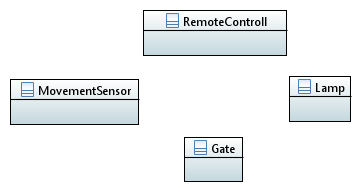
\includegraphics[width=100mm, keepaspectratio]{figures/component.png}
	\caption{Garage gate components}
	\label{fig:Garage Component}
\end{figure}

These components can communicate to each other directly. The possible communication messages is shown on the \figref{Garage communication}

\begin{figure}[!ht]
	\centering
	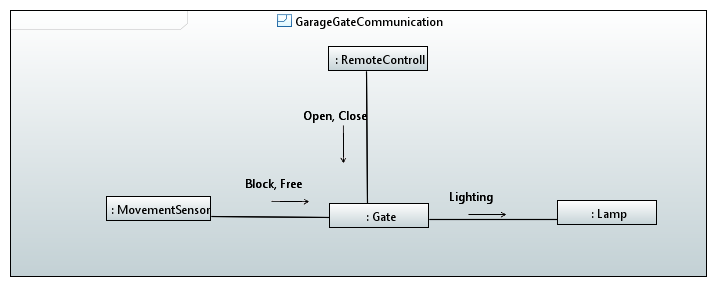
\includegraphics[width=150mm, keepaspectratio]{figures/communication.png}
	\caption{Garage gate communication diagram}
	\label{fig:Garage communication}
\end{figure}

A garage gate fundamentally have 2 main states, the \textit{Opened} and \textit{Closed} states, which is shown below on \figref{Garage Statemachine} figure, with orange colours.  First of all we can start from the \textit{Closed} state, where we can open the gate with an 'open' command. This command sets the state machine in an \textit{Opening} state. While opening the gate, somebody or something can move into the way, so this becomes \textit{Block Opening}. The gate is opening, if the blocking stops. After the \textit{Opening} phase succeeded the gate is \textit{Opened}. In this state we can 'close' the gate with a simple command, and the state machine goes to the \textit{Closing} state. There could be also a blocking action, which stops the closing movement. From this state the gate is starting the closing movement again after a few seconds \textit{Lighting}. When the closing action finished the gate is \textit{Closed}.



\begin{figure}[!ht]
\centering
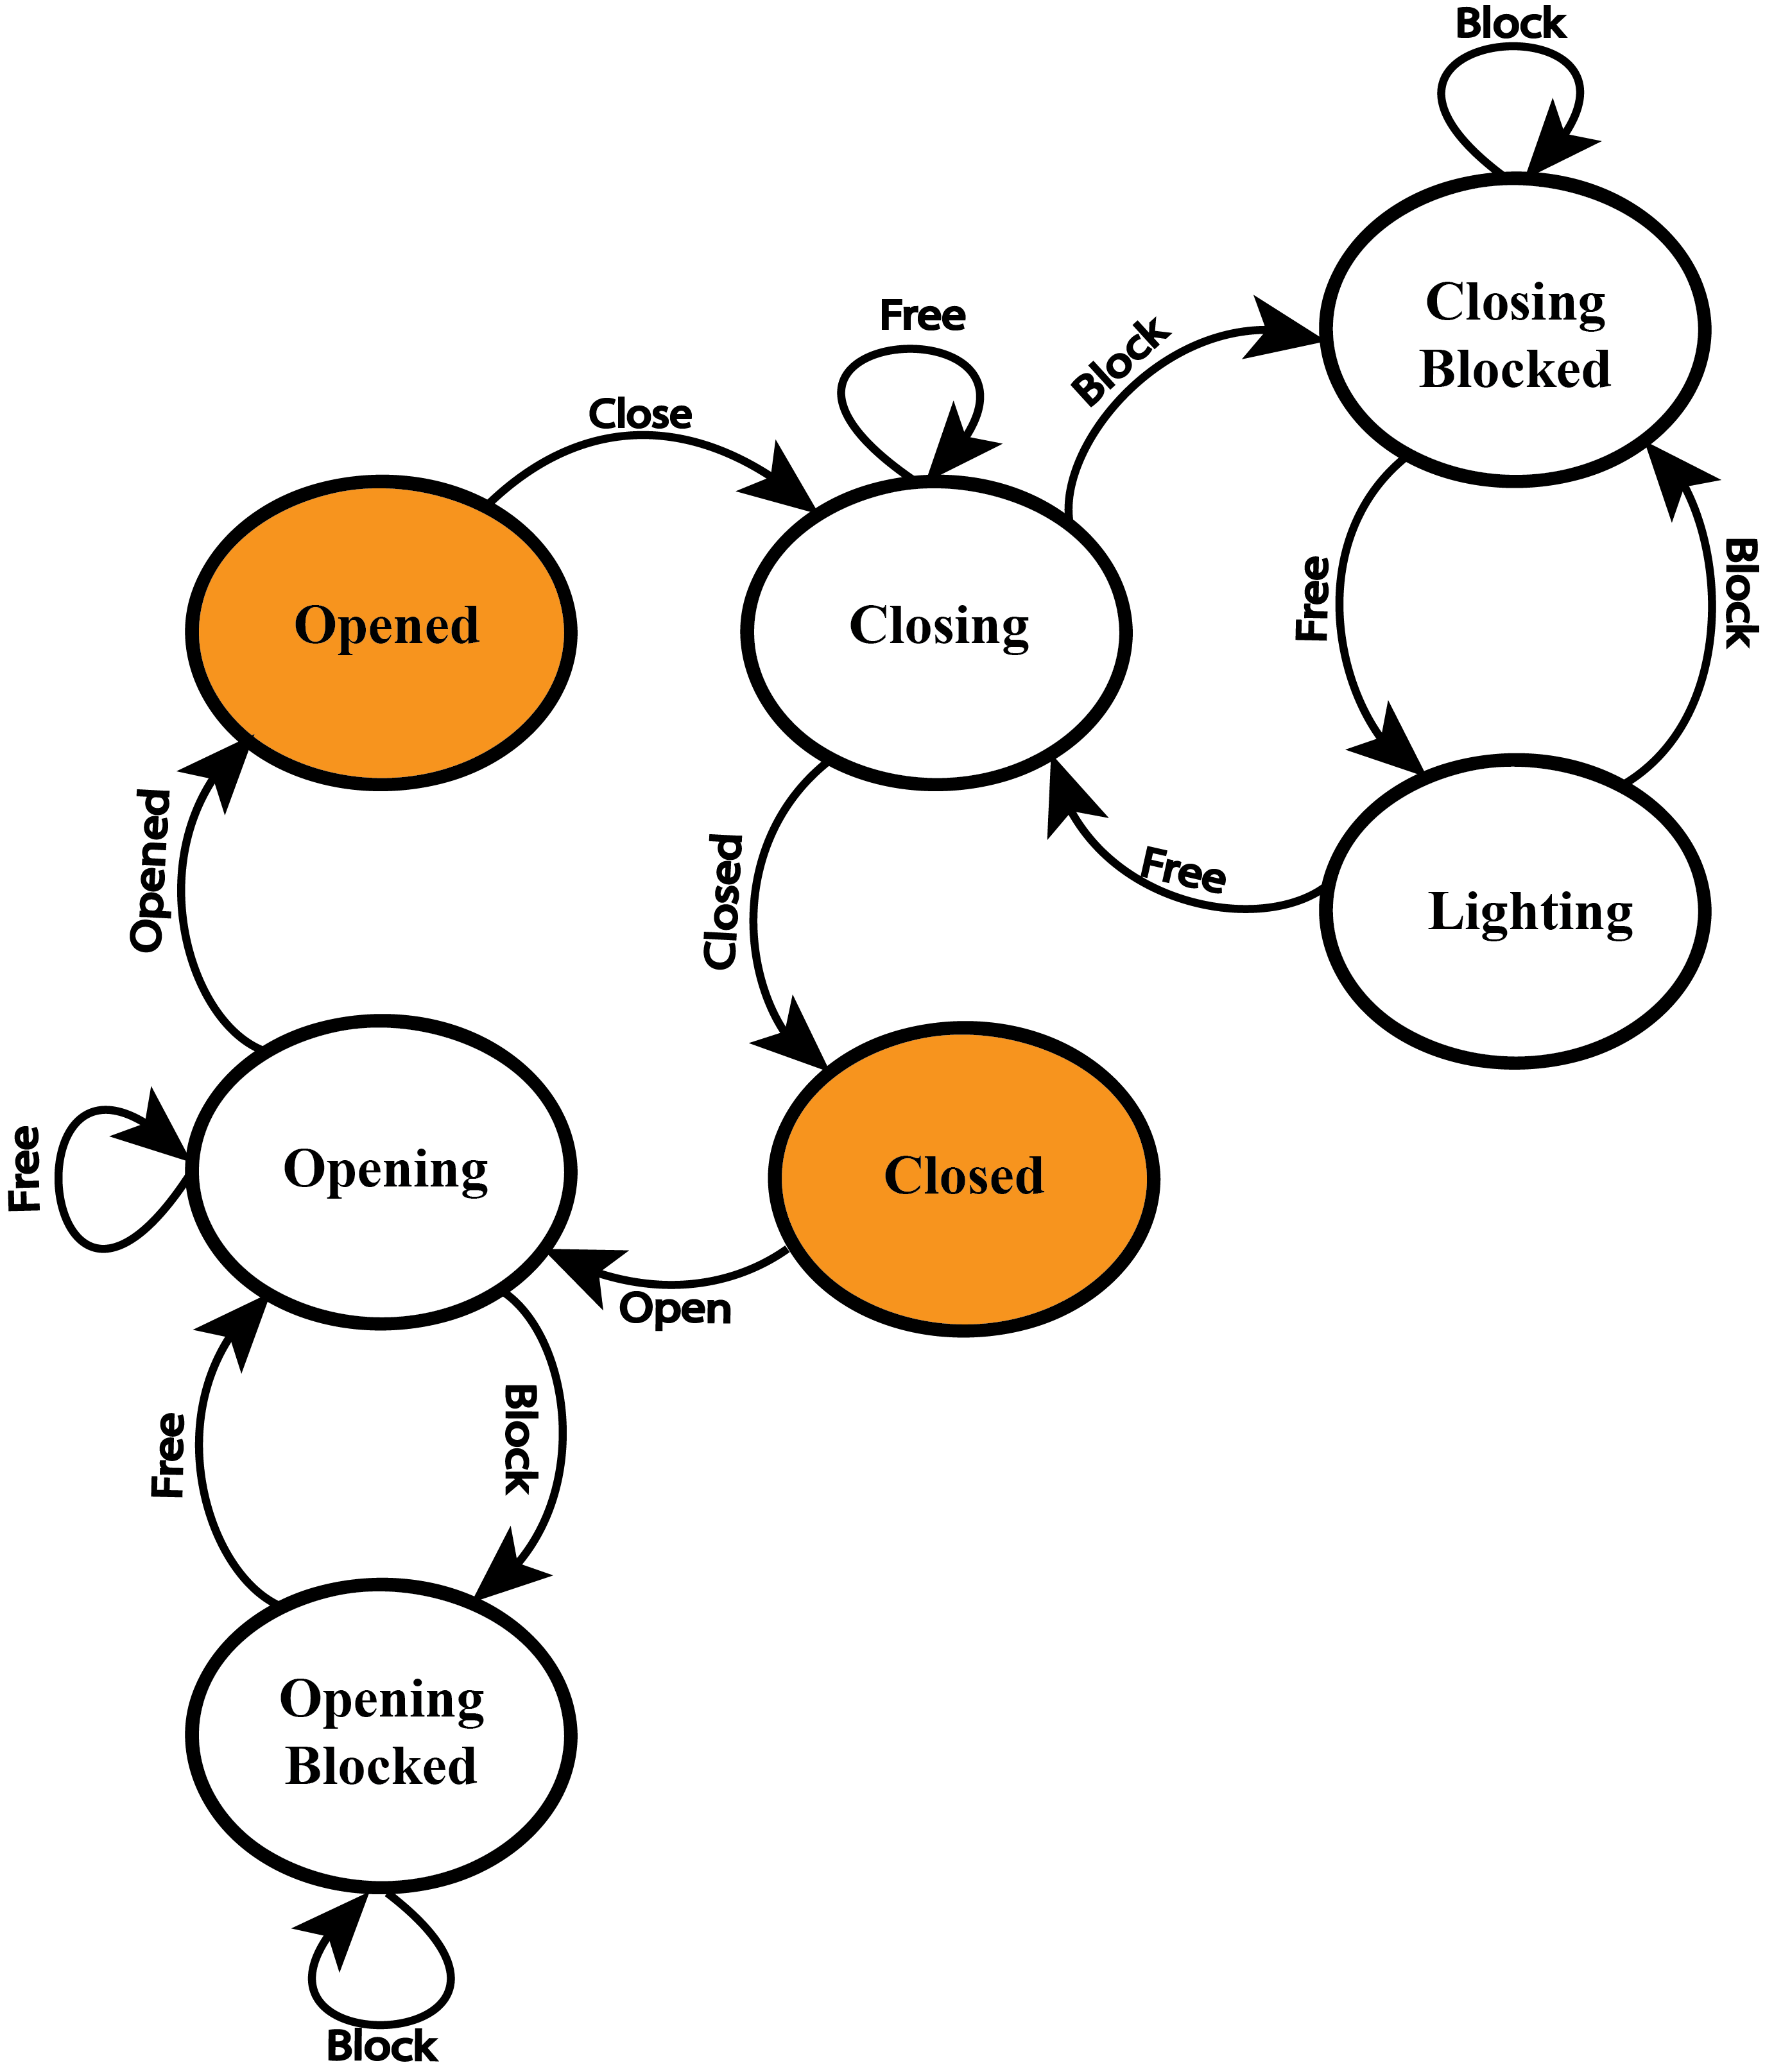
\includegraphics[width=150mm, keepaspectratio]{figures/garageState.png}
\caption{Garage gate state machine diagram}
\label{fig:Garage Statemachine}
\end{figure}


%----------------------------------------------------------------------------
\chapter{GraphWalker}\label{sect:GraphWalker implementation of Garage Gate model}

%----------------------------------------------------------------------------
\section{GraphWalker}
%----------------------------------------------------------------------------

\section{GraphWalker implementation in Eclipse}

 We can connect more models with the \textit{SHARED:someName} keyword in a vertex. Consequently I have created a yEd graph model for test scenarios for the garage gate state machine (see \figref{Garage Statemachine}), and a graph model for the lamp, which called from the previous graph.

\begin{figure}[!ht]
	\centering
	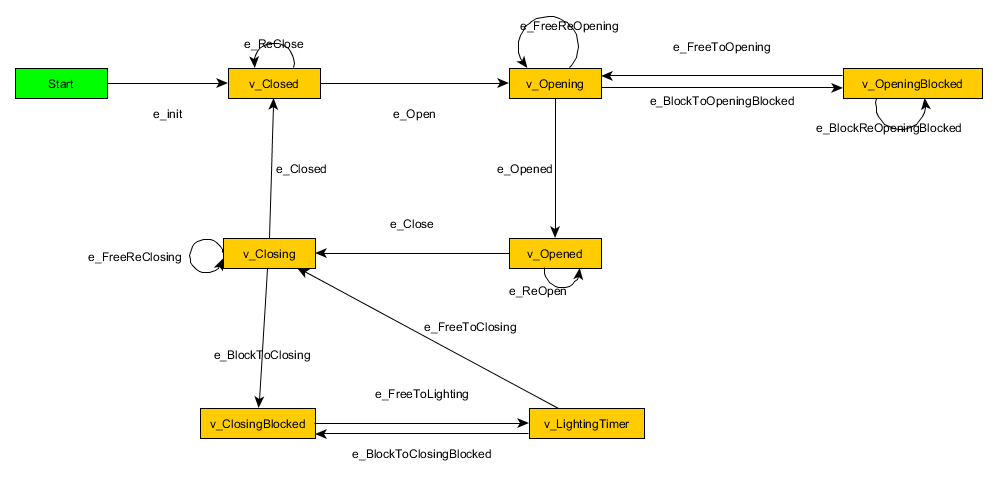
\includegraphics[width=150mm, keepaspectratio]{figures/GateModel.png}
	\caption{Garage gate model with yEd}
	\label{fig:GateModel}
\end{figure}

\begin{figure}[!ht]
	\centering
	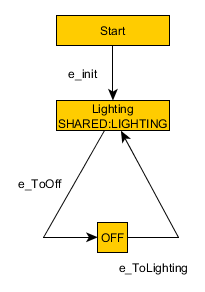
\includegraphics[width=50mm, keepaspectratio]{figures/LightingModel.png}
	\caption{Lamp0 model with yEd}
	\label{fig:LampModel}
\end{figure}


Generated test with option: @GraphWalker(start = "e\_init", value = "random(vertex\_coverage(100))"), and the result was:
[INFO] Result :
[INFO] 
[INFO] {
	"totalFailedNumberOfModels": 0,
	"totalNotExecutedNumberOfModels": 0,
	"totalNumberOfUnvisitedVertices": 0,
	"verticesNotVisited": [],
	"totalNumberOfModels": 2,
	"totalCompletedNumberOfModels": 2,
	"totalNumberOfVisitedEdges": 14,
	"totalIncompleteNumberOfModels": 0,
	"edgesNotVisited": [
	{
		"modelName": "GateModel",
		"edgeId": "e0",
		"edgeName": "e\_init"
	},
	{
		"modelName": "GateModel",
		"edgeId": "e3",
		"edgeName": "e\_Close"
	},
	{
		"modelName": "GateModel",
		"edgeId": "e10",
		"edgeName": "e\_FreeToOpening"
	},
	{
		"modelName": "GateModel",
		"edgeId": "e13",
		"edgeName": "e\_BlockReOpeningBlocked"
	}
	],
	"vertexCoverage": 100,
	"totalNumberOfEdges": 18,
	"totalNumberOfVisitedVertices": 9,
	"edgeCoverage": 77,
	"totalNumberOfVertices": 9,
	"totalNumberOfUnvisitedEdges": 4
}

%TODO implement PyModel stuff
\section{PyModel implementation}

% Acknowledgements, Köszönetnyilvánítás
%~~~~~~~~~~~~~~~~~~~~~~~~~~~~~~~~~~~~~~~~~~~~~~~~~~~~~~~~~~~~~~~~~~~~~~~~~~~~~~~~~~~~~~
%%----------------------------------------------------------------------------
\chapter*{\koszonetnyilvanitas}\addcontentsline{toc}{chapter}{\koszonetnyilvanitas}
%----------------------------------------------------------------------------

Ez nem kötelező, akár törölhető is. Ha a szerző szükségét érzi, itt lehet köszönetet nyilvánítani azoknak, akik hozzájárultak munkájukkal ahhoz, hogy a hallgató a szakdolgozatban vagy diplomamunkában leírt feladatokat sikeresen elvégezze. A konzulensnek való köszönetnyilvánítás sem kötelező, a konzulensnek hivatalosan is dolga, hogy a hallgatót konzultálja.


% List of Figures, Tables
%~~~~~~~~~~~~~~~~~~~~~~~~~~~~~~~~~~~~~~~~~~~~~~~~~~~~~~~~~~~~~~~~~~~~~~~~~~~~~~~~~~~~~~
\listoffigures\addcontentsline{toc}{chapter}{\abrakjegyzeke}
\listoftables\addcontentsline{toc}{chapter}{\tablazatokjegyzeke}


% Bibliography
%~~~~~~~~~~~~~~~~~~~~~~~~~~~~~~~~~~~~~~~~~~~~~~~~~~~~~~~~~~~~~~~~~~~~~~~~~~~~~~~~~~~~~~
%\bibliography{bib/mybib}
%\addcontentsline{toc}{chapter}{\irodalomjegyzek}


% Appendix
%~~~~~~~~~~~~~~~~~~~~~~~~~~~~~~~~~~~~~~~~~~~~~~~~~~~~~~~~~~~~~~~~~~~~~~~~~~~~~~~~~~~~~~
%----------------------------------------------------------------------------
\appendix
%----------------------------------------------------------------------------
\chapter*{\fuggelek}\addcontentsline{toc}{chapter}{\fuggelek}
\setcounter{chapter}{\appendixnumber}
%\setcounter{equation}{0} % a fofejezet-szamlalo az angol ABC 6. betuje (F) lesz
\numberwithin{equation}{section}
\numberwithin{figure}{section}
\numberwithin{lstlisting}{section}
%\numberwithin{tabular}{section}


%\label{page:last}
\end{document}
